\section{Introduction}
\hspace*{0.16in}

\section{ALL-IDB}

ALL-IDB (Acute Lymphoblastic Leukemia Image Database for Image Processing) \textsuperscript{\cite{labati2011all}} is a public and free dataset, specifically designed for the evaluation and the comparison of algorithms for segmentation and image classification. The database focus on Acute Lymphoblastic Leukemia (ALL), Acute is a type of blood cancer that starts in white blood cells in bone marrow, the soft inner part of bones. It develops from immature lymphocytes, a kind of white blood cell that’s key to immune system.\textsuperscript{\cite{Annie_Stuart_What_2022_webmd}}.\\

Each image in the dataset, Contains classification/position of ALL lymphoblasts is provided by expert oncologists. A lymphoblast is a modified naive lymphocyte with altered cell morphology. It occurs when the lymphocyte is activated by an antigen.\\

The images of the dataset has been captured with an optical laboratory microscope coupled with a Canon PowerShot G5 camera. All images are in JPG format with 24 bit color depth, resolution 2592 x 1944. the ALL-IDB devides on two Datasets ALL-IDB1 and ALL-IDB2.\\

\subsection{Dataset ALL-IDB1}

The ALL-IDB1 can be used for segmentation or classification with image processing methods or Artificial intelligence models. The dataset is composed of 108 images collected during September, 2005. It contains about 39000 blood elements, where the lymphocytes has been labeled by expert oncologists.

\begin{figure}[H]
\centering
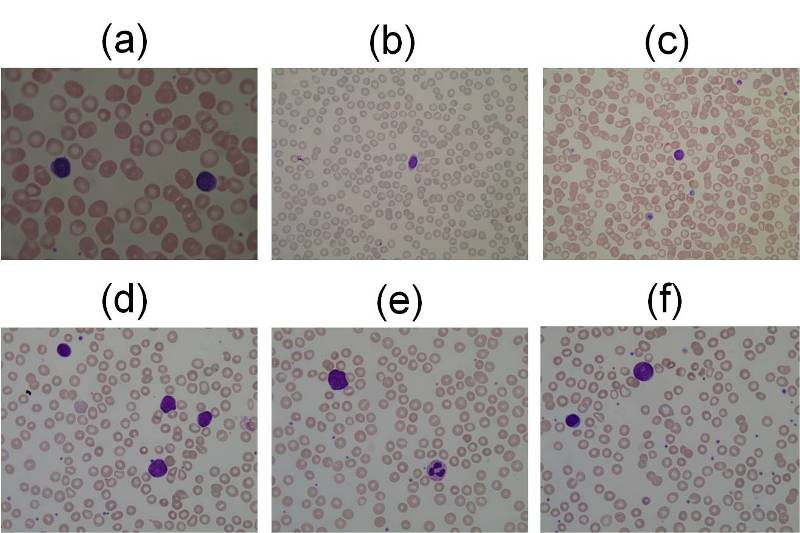
\includegraphics{ALLIDB1}
\caption{Examples of the images contained in ALL-IDB1: healthy cells from non-ALL patients (a,b,c), probable lymphoblasts from ALL patients (d,e,f). }
\end{figure}


\textbf{annotation:} input image ''Im006\_1.jpg'' (a) and the related classification file ''Im006\_1.xyc'' reporting the coordinates of the centroids of probable ALL lymphoblasts (b).



\begin{figure}[H]
\begin{minipage}[b]{0.35\linewidth}
\centering
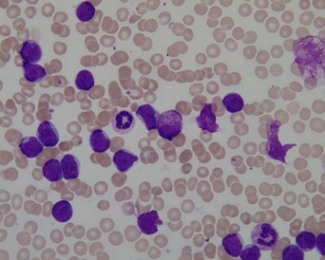
\includegraphics{Im006_1}
\subcaption{Im006\_1.jpg}
\label{fig:Im006.jpg}
\end{minipage}
\hfill
\begin{minipage}[b]{0.3\linewidth}
\centering
\lstinputlisting[breaklines]{images/Im006\_1.xyc}
\subcaption{Im006\_1.xyc}
\label{fig:Im006.xyc}
\end{minipage}

\begin{minipage}[b]{0.35\linewidth}
\centering
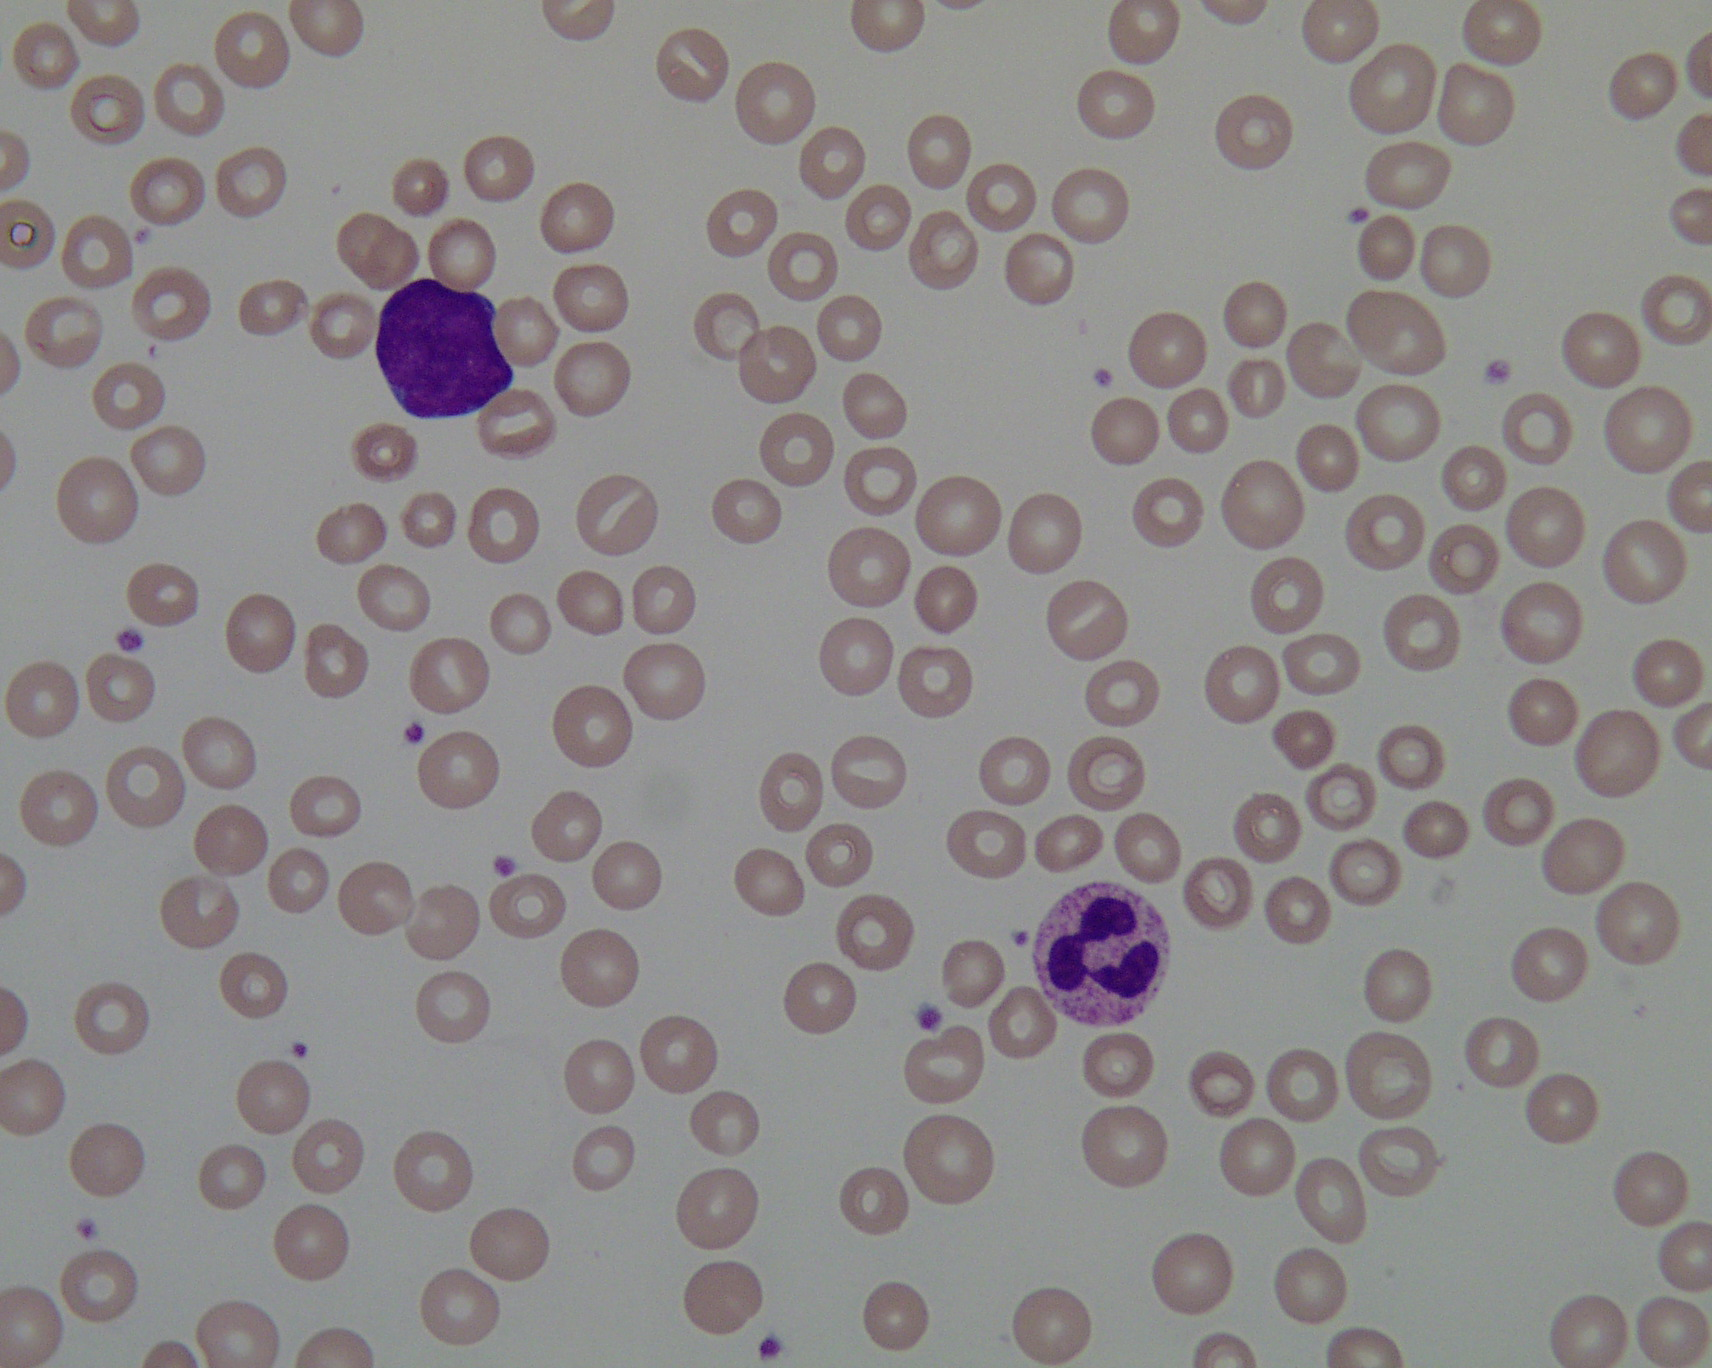
\includegraphics[width=57mm]{Im033_1}
\subcaption{Im033\_1.jpg}
\label{fig:Im033.jpg}
\end{minipage}
\hfill
\begin{minipage}[b]{0.3\linewidth}
\centering
\lstinputlisting[breaklines]{images/Im033\_1.xyc}
\subcaption{Im033\_1.xyc}
\label{fig:Im033.xyc}
\end{minipage}
\caption{Sample data from the ALL-IDB1 Database}
\end{figure}

The ALL-IDB1 image files are named with the notation ImXXX\_Y.jpg where XXX is a 3-digit integer counter and Y is a boolean digit equal to 0 if no blast cells are present, and equal to 1 if at least one blast cell is present in the image. All images labeled with Y=0 are from for healthy individuals, and all images labeled with Y=1 are from ALL patients. Each image file ImXXX\_Y.jpg (figure \ref{fig:Im006.jpg}, \ref{fig:Im033.jpg}) is associated with a text file ImXXX\_Y.xyc (figure \ref{fig:Im006.xyc}, \ref{fig:Im033.xyc}) reporting the coordinates of the centroids of the blast cells, if any. \\

if we plot the coordinates in the Img006\_1.xyc (figure \ref{fig:Im006.jpg}) file on the image Im006\_1.jpg (figure \ref{fig:Im006.xyc}) we get the figure \ref{fig:Im006.xyc.jpg}

\begin{figure}[H]
\centering
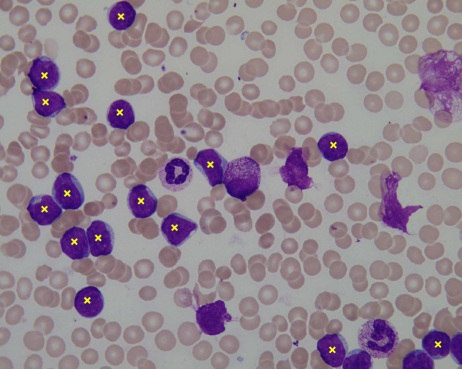
\includegraphics{images/img006.xyc.jpg}
\caption{coordinates from Img006\_1.xyc ploted on Img006\_1.jpg}
\label{fig:Im006.xyc.jpg}
\end{figure}

\newpage

\subsection{Dataset ALL-IDB1}

This dataset has been created for testing the performances of classification systems. where the dataset has no segmentation information it contains only one information wich is the presence of ALL lymphoblasts, the dataset is a collection of cropped area of interest of normal and blast cells that belongs to the ALL-IDB1 dataset as we can see in figure \ref{fig:ALL-IDB2}


\begin{figure}[H]
\centering
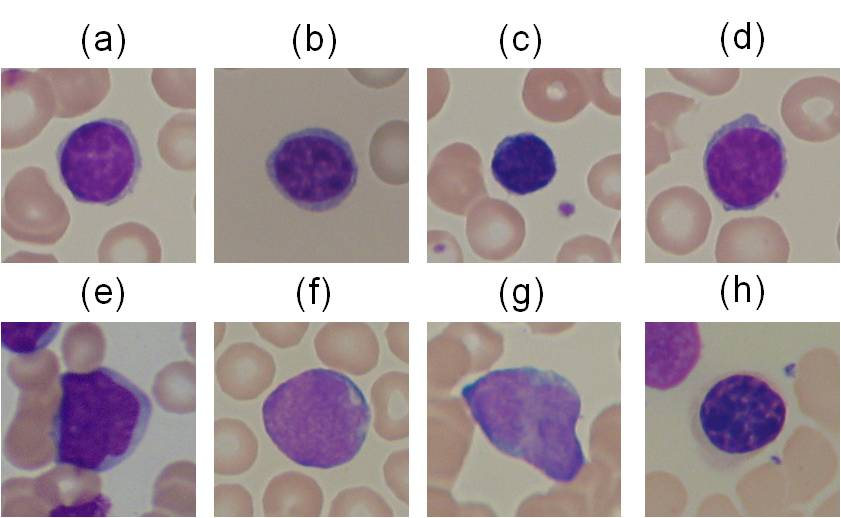
\includegraphics{images/ALL-IDB2.jpg}
\caption{Examples of the images contained in ALL-IDB2: healthy cells from non-ALL patients (a-d), probable lymphoblasts from ALL patients (e-h).}
\label{fig:ALL-IDB2}
\end{figure}


The annotation of ALL-IDB2 is similar to the ALL-IDB1 but with no centroid coordinates. The ALL-IDB2 image files are named with the notation ImXXX\_Y.jpg where XXX is a progressive 3-digit integer and Y is a boolean digit equal to 0 if the cell placed in the center of the image is not a blast cell, and equal to 1 if the cell placed in the center of the image is a blast cell. all images labeled with Y=0 are from for healthy individuals, and all images labeled with Y=1 are from ALL patients. 

\newpage 

\section{Conclusion}
\hspace*{0.16in}

\newpage